\chapter{Estudo de viabilidade}\label{sec:EstuViab}
O estudo de viabilidade constitui-se como uma etapa metodológica essencial no processo de desenvolvimento de sistemas de informação, caracterizado pela análise sistemática e multidimensional dos aspectos técnicos, operacionais, econômicos e temporais que determinam a exequibilidade de um projeto de software \cite{pressman2014software}. Esta fase investigativa visa identificar potenciais obstáculos, avaliar recursos necessários, estimar custos e benefícios, e determinar a probabilidade de sucesso da implementação proposta antes do comprometimento significativo de recursos organizacionais e humanos \cite{sommerville2016engineering}.

A importância do estudo de viabilidade fundamenta-se na necessidade de tomada de decisão informada sobre a continuidade ou descontinuidade de projetos de desenvolvimento, evitando investimentos em iniciativas que apresentem barreiras intransponíveis ou relação custo-benefício desfavorável \cite{kendall2014systems}. No contexto acadêmico e de inovação tecnológica, esta análise assume relevância adicional ao permitir a identificação precoce de limitações técnicas, restrições de recursos, e desafios de implementação que possam comprometer os objetivos do projeto.

O estudo de viabilidade tipicamente abrange quatro dimensões fundamentais de análise. A viabilidade técnica examina se os recursos tecnológicos, conhecimentos especializados e infraestrutura necessários estão disponíveis ou podem ser adquiridos para a implementação bem-sucedida do sistema \cite{whitten2003systems}. A viabilidade operacional avalia se o sistema proposto será aceito e efetivamente utilizado pelos usuários finais, considerando aspectos de usabilidade, adequação ao contexto de uso e alinhamento com as necessidades reais dos stakeholders \cite{dennis2015systems}. A viabilidade econômica analisa a relação entre custos de desenvolvimento, implementação e manutenção frente aos benefícios tangíveis e intangíveis que o sistema proporcionará \cite{marakas2006systems}. Por fim, a viabilidade temporal examina se o projeto pode ser concluído dentro de prazos aceitáveis e se sua implementação ocorrerá em momento oportuno para atender às demandas identificadas.
\begin{comment}

No contexto específico do desenvolvimento da aplicação SheSafe, o estudo de viabilidade assume importância crítica ao considerar que se trata de um sistema voltado à segurança pessoal e resposta a situações de emergência. A análise deve contemplar não apenas os aspectos técnicos convencionais de desenvolvimento de aplicações móveis, mas também considerações especiais relacionadas à confiabilidade do sistema em situações críticas, proteção de dados sensíveis dos usuários, integração com recursos nativos do dispositivo móvel (como geolocalização e comunicação), e adequação da solução às necessidades reais de pessoas em situação de vulnerabilidade.
\end{comment}

A realização criteriosa do estudo de viabilidade proporciona múltiplos benefícios ao projeto, incluindo a identificação antecipada de riscos e desafios técnicos, o estabelecimento de expectativas realistas quanto a prazos e recursos necessários, a fundamentação para decisões de design e arquitetura do sistema, e a documentação das premissas e restrições que orientarão o desenvolvimento \cite{hughes2016project}. Esta análise sistemática contribui para aumentar as probabilidades de sucesso do projeto ao garantir que todos os aspectos críticos tenham sido devidamente considerados antes do início da implementação propriamente dita.

\section{Tipos de instrumento utilizados para a coleta de dados}
Foi utilizado para coleta de dados a abordagem de questionário com algumas perguntas distribuídas em quatro seções sendo elas idade/localidade, segurança, aplicativo SheSafe e comentários. 
A seção de idade e localidade continham perguntas relacionadas a idade dos usuários e a localidade, neste caso o estado, no qual eles vivem.
A seção de segurança abordou perguntas sobre a percepção do entrevistado em relação a questões como medo de sair na rua à noite, sobre já ter sofrido algum tipo de violência, entre outras perguntas que serão apresentadas na análise da coleta de dados.
A seção sobre o aplicativo SheSafe abordou perguntas quanto ao uso de um app que fosse capaz de ajudar aos entrevistados quando estivessem passando por uma situação adversa ou de risco. Também foram feitas perguntas sobre quais funcionalidades gostariam de ver em um aplicativo como este.
A seção de comentários ficou aberta para que os entrevistados pudessem expressar suas ideias e sugestões sobre a iniciativa do aplicativo SheSafe.
Tal instrumento foi escolhido por julgar que alcançaria mais pessoas, pois seria disponibilizado através de redes sociais.

\section{Abordagem e período de coleta}
O questionário foi disponibilizado por meio de um post no LinkedIn e por meio de divulgação em grupos de aplicativos de mensagens instantâneas desde o dia 24 de fevereiro de 2024 até o dia 9 de março de 2024. No post foi informado que o questionário era voltado para pessoas do sexo feminino.

\section{Questões utilizadas para a coleta de dados}
\begin{itemize}
  \item Idade e estado onde reside
  \item Já deixou de ir a algum lugar com medo de não ser seguro para você pelo fato de ser mulher?
  \item Você se sente segura ao andar na rua?
  \item Do que você mais tem medo quando sai sozinha à noite?
  \item Você já foi vítima de algum tipo de violência ou assédio?
  \item Você usaria um aplicativo que informasse se um determinado local possui alto índice de crimes relacionados a mulher ou até mesmo o quão esse lugar é seguro para mulheres?
  \item Quais funcionalidades você gostaria de ver em um aplicativo como este?
  \item Se você tiver algum outro comentário ou sugestão, por favor, escreva aqui:
\end{itemize}

\section{Resultados Obtidos}
\subsection{Idade e Localidade}
A primeira pergunta realizada foi sobre a idade do usuário, que com base no gráfico abaixo, podemos ver que a predominância foi entre as pessoas mais jovens. Pessoas mais jovens costumam utilizar mais tecnologia como meio de comunicação, sendo assim o maior alcance a esse grupo. 
\begin{figure}[H]
  \begin{center}
  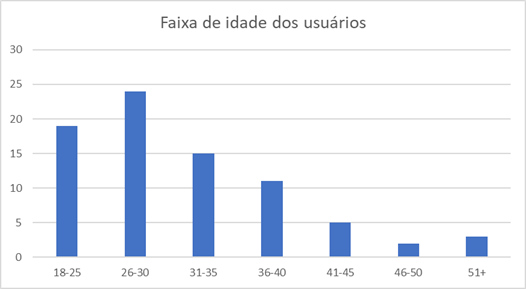
\includegraphics[width=0.6\linewidth]{images/distribuicao-idade.png}\\
  \end{center}
  \caption[Distribuição de faixa etária]{Distribuição de faixa etária}
  \label{fig:mapa-empatia=inicial}
  \legend{Fonte: Próprio Autor}
\end{figure}

A segunda pergunta foi quanto a localidade (estado) em que o entrevistado mora. Pelo gráfico abaixo, podemos ver que a maior parte dos entrevistados foram oriundos do estado de São Paulo. Embora a pesquisa não tenha conseguido coletar dados e pessoas de alguns estados, podemos ver que conseguimos abranger uma boa parte dos estados brasileiros.
\begin{figure}[H]
  \begin{center}
  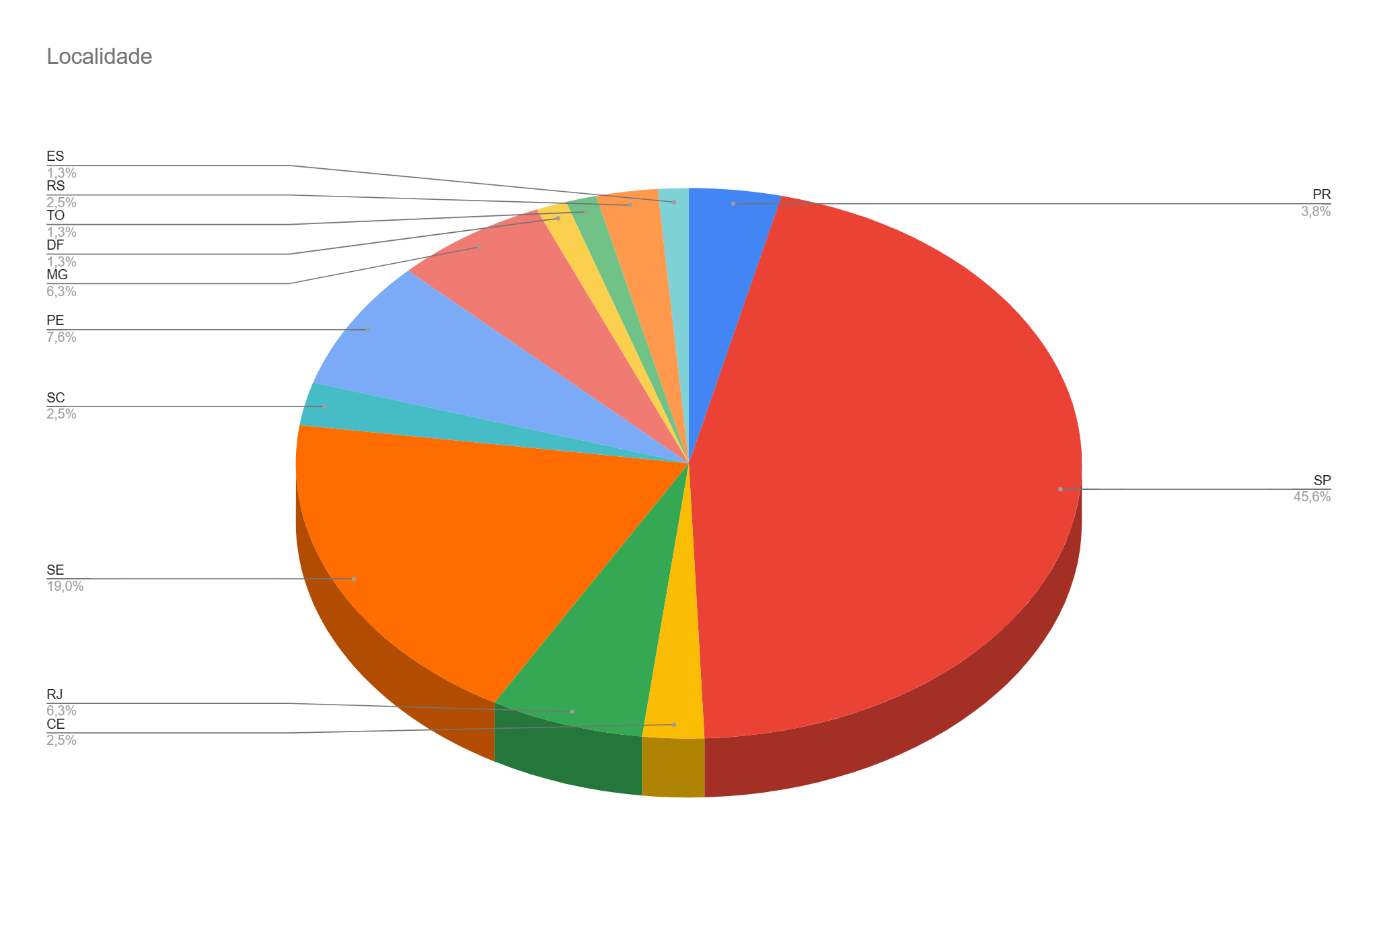
\includegraphics[width=0.6\linewidth]{images/distribuicao-estados.png}\\
  \end{center}
  \caption[Distribuição de localização]{Distribuição de localização}
  \label{fig:mapa-empatia=inicial}
  \legend{Fonte: Próprio Autor}
\end{figure}

\subsection{Segurança}
A primeira pergunta relacionada a segurança foi quanto ao fato do entrevistado se privar de ir a lugares por conta de ser uma mulher. O gráfico abaixo nos mostra, que infelizmente, muitas mulheres ainda se privam de ir a determinados lugares por conta do medo do que pode acontecer a elas, simplesmente por serem mulheres. 
\begin{figure}[H]
  \begin{center}
  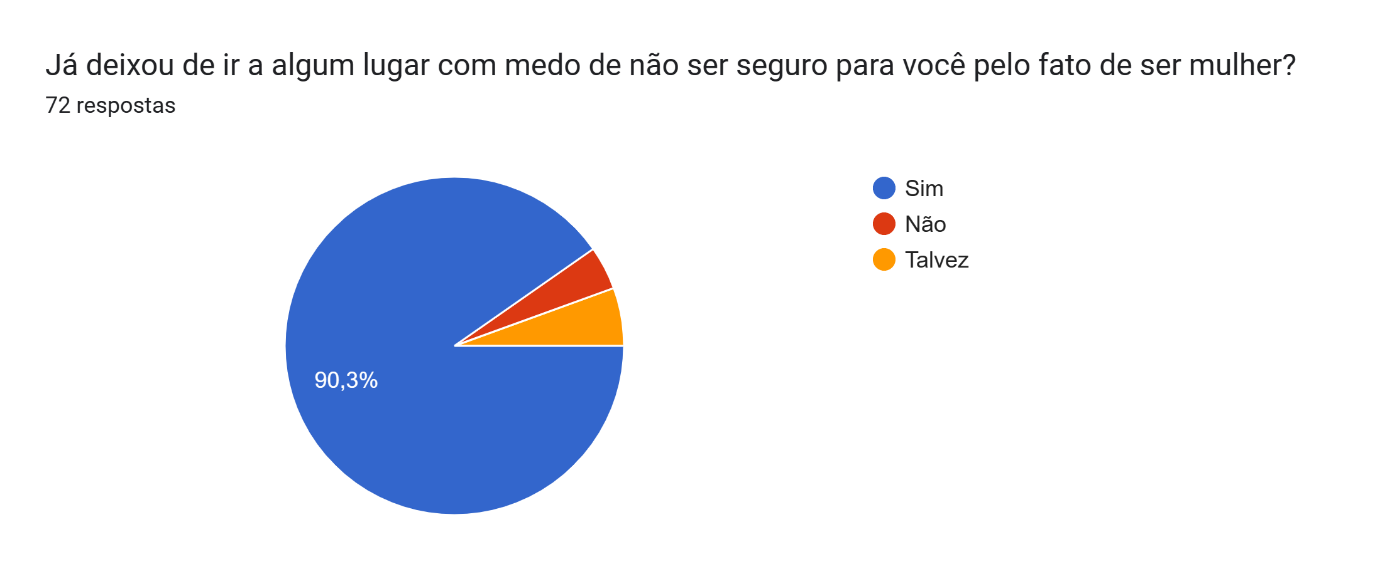
\includegraphics[width=1.0\linewidth]{images/distribuicao-privacao-mulher.png}\\
  \end{center}
  \caption[Distribuição de privação de local]{Distribuição de privação de local}
  \label{fig:mapa-empatia=inicial}
  \legend{Fonte: Próprio Autor}
\end{figure}
%\clearpage

A segunda pergunta foi sobre o entrevistado se sentir seguro ao andar na rua. O resultado abaixo nos mostra que majoritariamente as mulheres não se sentem seguras ao andar na rua. Tendo o receio de andar na rua em determinados lugares. 
\begin{figure}[H]
  \begin{center}
  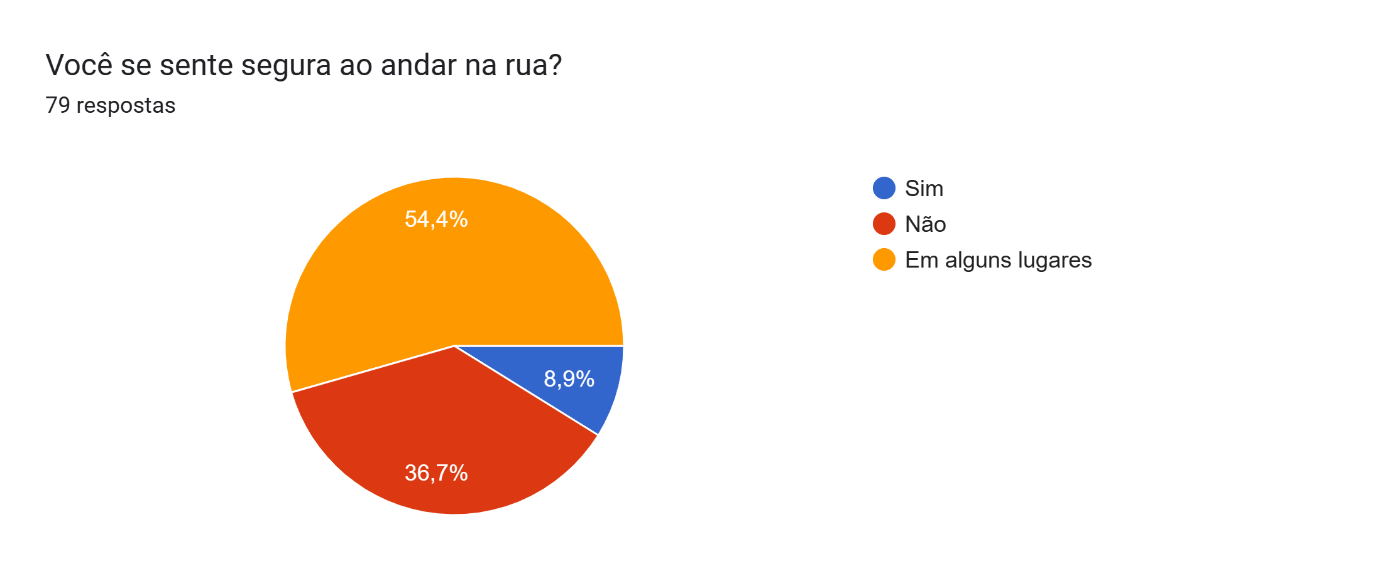
\includegraphics[width=1.0\linewidth]{images/distribuicao-seguranca-rua.png}\\
  \end{center}
  \caption[Distribuição de sentimento de segurança]{Distribuição de sentimento de segurança}
  \label{fig:mapa-empatia=inicial}
  \legend{Fonte: Próprio Autor}
\end{figure}
%\clearpage

A terceira pergunta desta seção foi relacionada ao tipo de medo que a mulher sentia ao sair à noite sozinha. A pergunta poderia ter várias respostas escolhidas e os resultados abaixo nos mostram que a violência ainda continua sendo o principal medo reportado por elas.
\begin{figure}[H]
  \begin{center}
  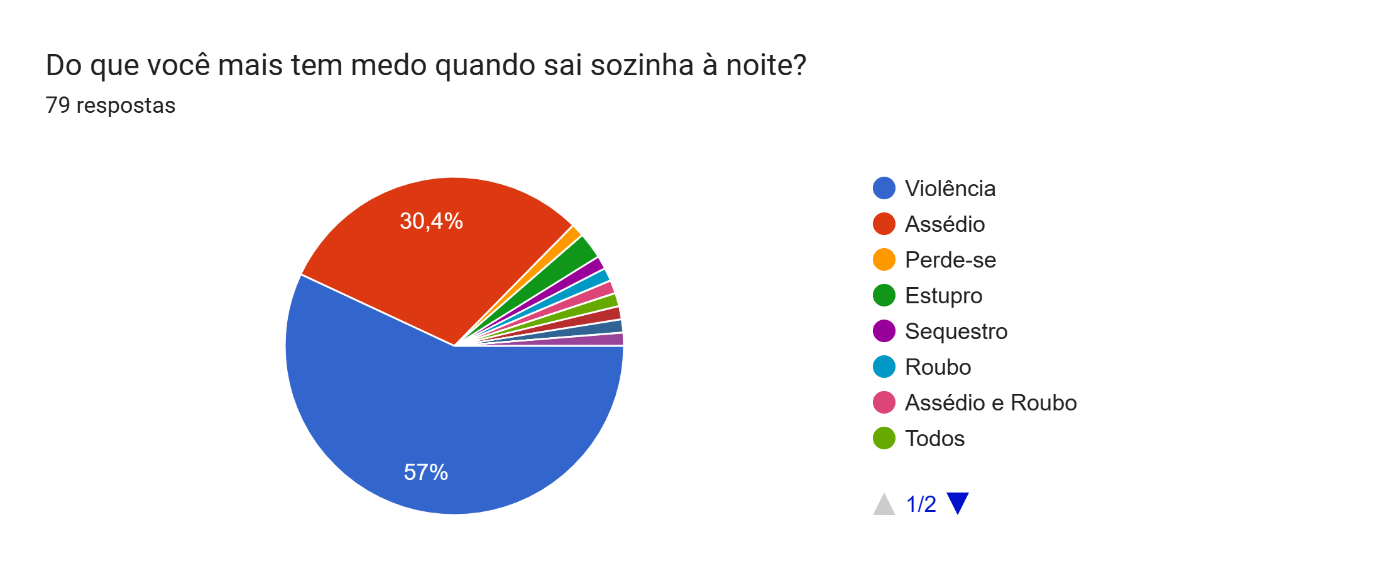
\includegraphics[width=0.5\linewidth]{images/distribuicao-medo.png}\\
  \end{center}
  \caption[Distribuição de maior medo]{Distribuição de maior medo}
  \label{fig:mapa-empatia=inicial}
  \legend{Fonte: Próprio Autor}
\end{figure}
%\clearpage

A última pergunta da seção de segurança foi um pouco mais direta quanto ao fato da entrevistada já ter sofrido algum tipo de violência ou assédio. Mais uma vez, majoritariamente, podemos ver que infelizmente muitas mulheres já passaram por essas situações. 
\begin{figure}[H]
  %\begin{center}
  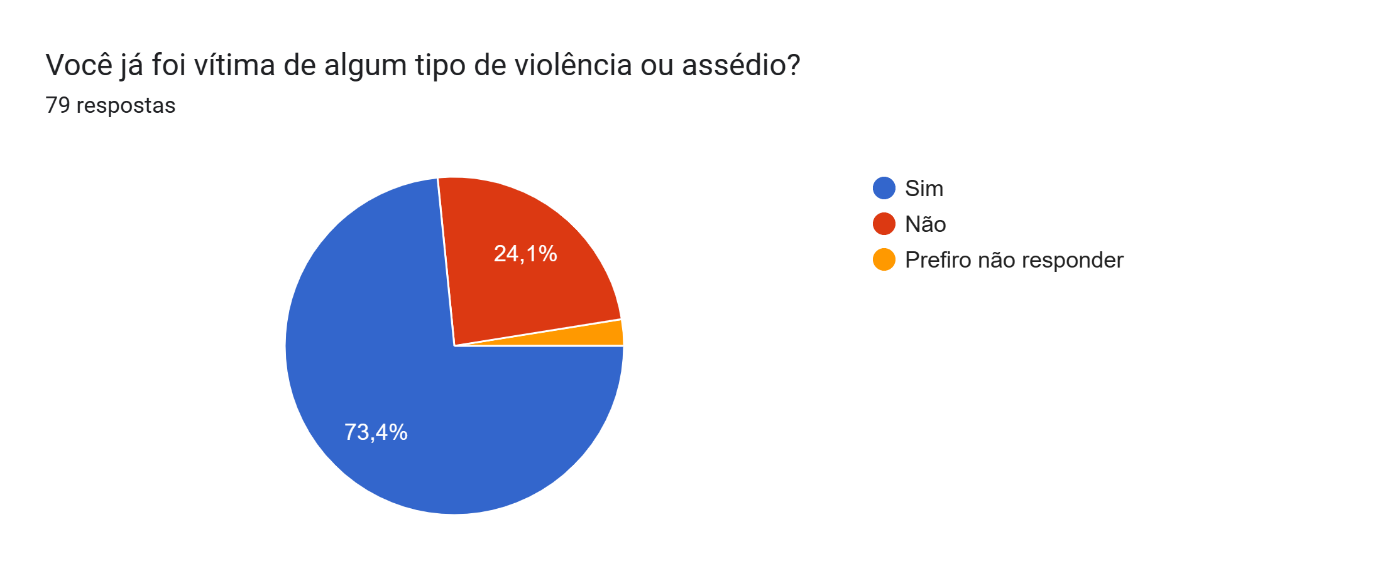
\includegraphics[width=0.5\linewidth]{images/distribuicao-vitma.png}\\
  %\end{center}
  \caption[Distribuição de vítima]{Distribuição de vítima}
  \label{fig:distribuicao-vitmal}
  \legend{Fonte: Próprio Autor}
\end{figure}
%\clearpage

\subsection{Uso do aplicativo}
A primeira pergunta nesta seção indagava aos entrevistados sobre o uso de um aplicativo capaz de mostrar informações sobre a segurança de um determinado local. Abaixo podemos ver no gráfico que os usuários percebem a utilidade em usar um aplicativo para tal fim.

\begin{figure}[h]
  \begin{center}
  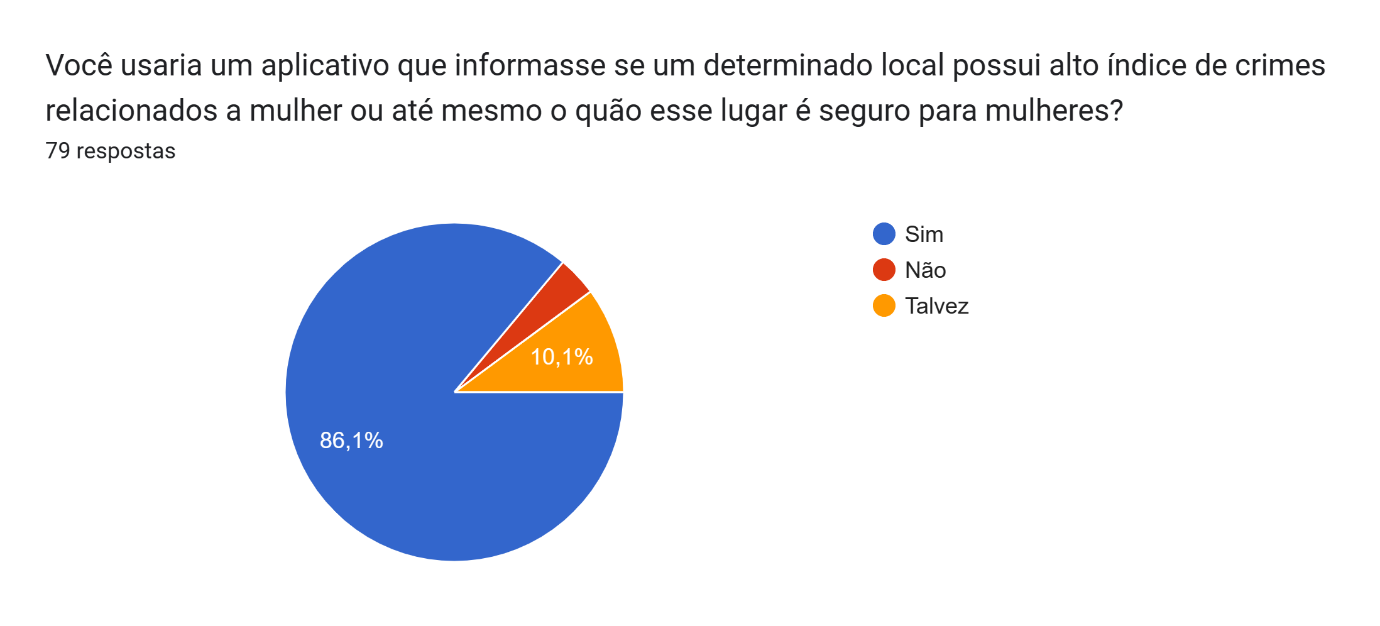
\includegraphics[width=1.0\linewidth]{images/distribuicao-uso-aplicativo.png}\\
  \end{center}
  \caption[Distribuição uso do aplicativo]{Distribuição uso do aplicativo}
  \label{fig:distribuicao-uso-aplicativo}
  \legend{Fonte: Próprio Autor}
\end{figure}

A segunda pergunta nesta seção focava sobre quais as funcionalidades que os usuários gostariam de ver no aplicativo. Abaixo é mostrado um resumo das escolhas dos usuários onde é possível notar que informações sobre segurança, forma de pedir ajuda e rastreamento em tempo real foram as funcionalidades mais votadas. As opções de respostas eram:
\begin{itemize}
  \item Informações sobre segurança do local
  \item Possibilidade de pedir ajuda em caso de emergência
  \item Rastreamento de localização
  \item Rede de apoio com outras mulheres
  \item Outros
\end{itemize}

\begin{figure}[h]
  \begin{center}
  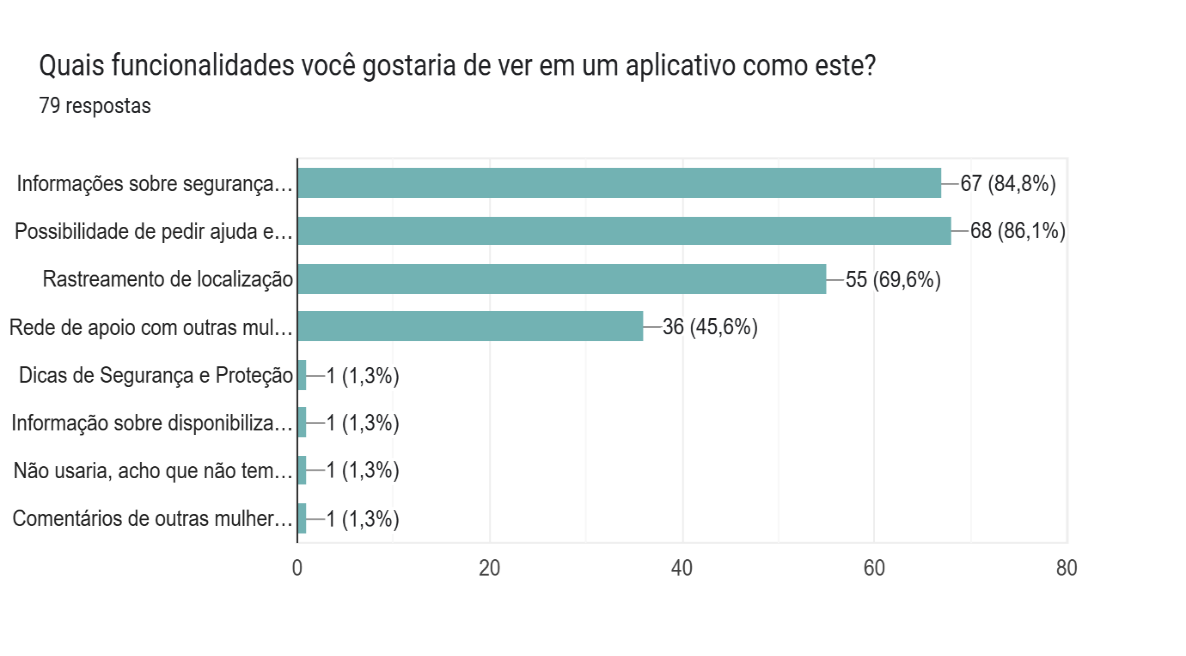
\includegraphics[width=1.0\linewidth]{images/distribuicao-escolha-funcionalidades.png}\\
  \end{center}
  \caption[Distribuição de escolha de funcionalidades]{Distribuição de escolha de funcionaldades}
  \label{fig:distribuicao-escolha-funcionalidades}
  \legend{Fonte: Próprio Autor}
\end{figure}

\subsection{Comentários gerais}
Foi adicionada uma seção em que os entrevistados podiam deixar suas opiniões e sugestões. Dando foco emalgumas opniões que foram relatas, foi possível perceber certas preocupações dos possíveis usuários do aplicativo. 

Um entrevistado escreveu o seguinte comentário: “Minha preocupação seria na possibilidade de criminosos utilizarem o aplicativo para terem acesso a essas mulheres, dependendo do tipo de funcionalidade implementada”. Realmente ao mesmo tempo em que temos que nos preocupar em disponibilizar uma ferramenta para ajudar nossos usuários, temos que garantir a segurança desta ferramenta, para que ela não acabe se tornando uma arma para criminosos.

Outro entrevistado escreveu: “Talvez informar que o local é inseguro nos traz mais insegurança do que o necessário. Muitas podem desencadear reações ruins como síndrome do pânico e ansiedade, até depressão e se isolar (não sou especialista), mas, por exemplo, deixo de assistir noticiários por excesso de notícias ruins nos deixar em pânico.”. A intenção é que a aplicação possa ajudar nossos usuários à terem menos receio quanto a segurança. A ideia de implementar um histórico sobre local ou até mesmo índice de criminalidade terá que ser amadurecida.

“Acredito que será de grande utilidade para levantamento de dados para a segurança pública, mas a maioria das vezes, a mulher TEM que ir ao lugar independente da informação... então não vejo um avanço significativo para a mulher diretamente, seria mais para levantamento de dados da segurança pública mesmo.” A fala desta entrevistada demonstra como hoje ainda há muito da cultura patriarcal. A intenção da ferramenta não é dizer aonde nosso usuário deve ir ou não, mas sim mostrar dados acerca da segurança de um determinado local. Este comentário corrobora com o comentário anterior sobre acabar criando algum tipo de síndrome no nosso usuário.

\section{Novo Personas e Mapa de empatia}
Dadas as informações coletadas podemos verificar que nossas suposições do mapa de empatia foram validadas em sua maior parte. Desta forma, alguns pontos puderam ser levantados e mapeados em um novo mapa muito parecido com o primeiro, porém contendo agora algumas entradas mais voltadas ao problema. Abaixo podemos ver os novos pontos adicionados ao nosso mapa de empatia.
\begin{figure}[h]
  \begin{center}
  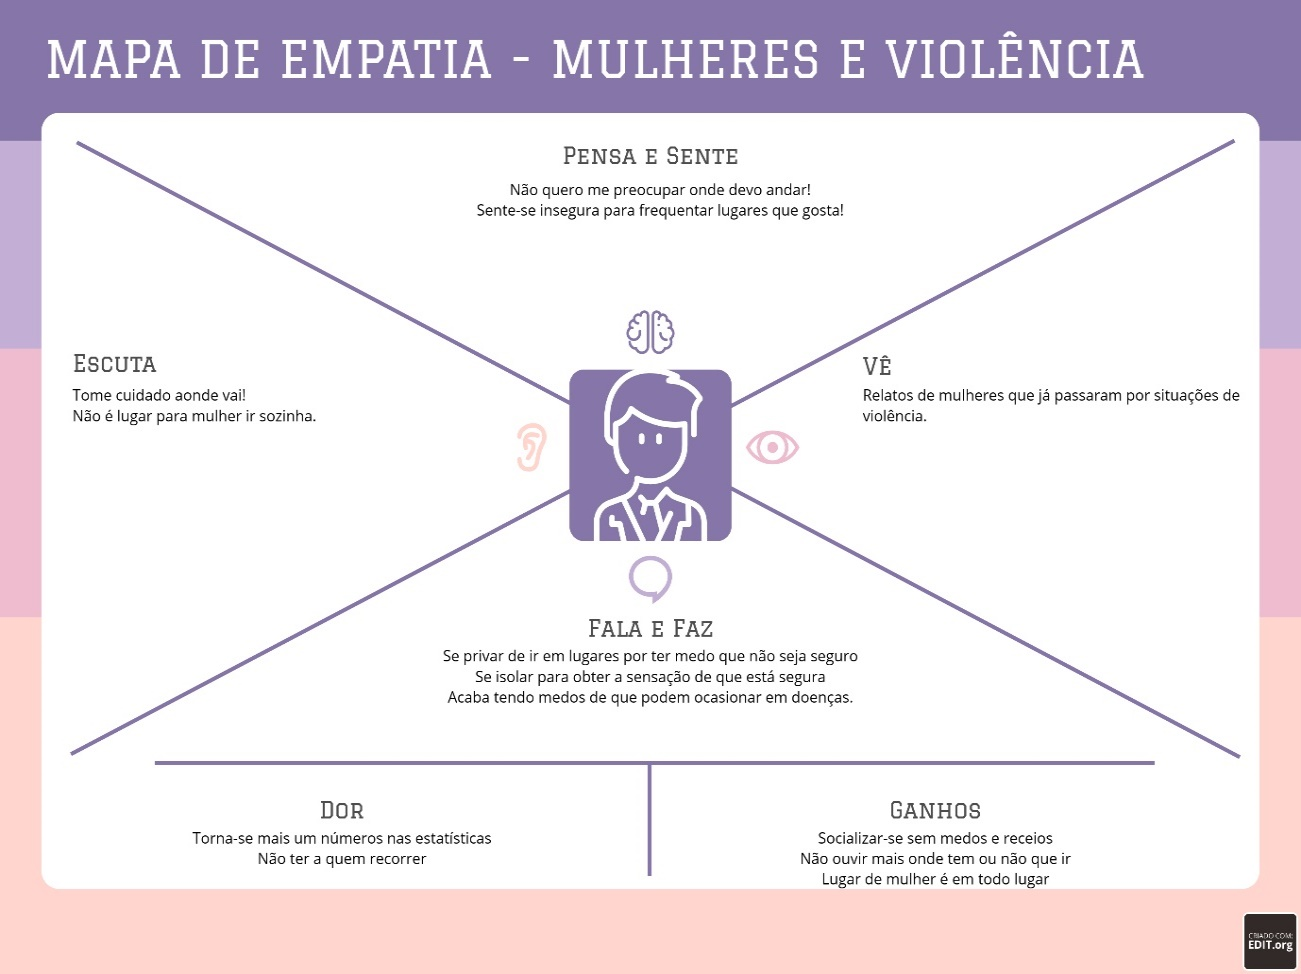
\includegraphics[width=1.0\linewidth]{images/mapa-empatia-novo.jpeg}\\
  \end{center}
  \caption[Nobo mapa de mepatia]{Novo mapa de empatia}
  \label{fig:novo-mapa-empatia}
  \legend{Fonte: Próprio Autor}
\end{figure}

Quanto ao nosso novo personas podemos agora enfatizar alguns pontos que antes não haviam ainda sido vistos em nossa análise.

Persona: Pessoas do sexo feminino de qualquer idade que em algum momento da vida já teve receio de sair de casa por medo da violência que pode ocorrer contra ela. São mulheres que desejam ter uma forma de pedir ajuda quando alguma situação estranha ou adversa estiver acontecendo com elas. São mulheres que não se sentem seguras ao sair de casa sozinha, pois acreditam que algo pode acontecer contra elas e não terão como pedir ajuda. Essas mulheres utilizam seus celulares no dia a dia para fazerem ligações, conversar por aplicativos de mensagens instantâneas e as até para pedir ajuda a pessoas as quais ela considera confiáveis. Em casos extremos, são mulheres que já sofreram ou sofrem algum tipo de violência, seja ela doméstica, verbal, moral ou até mesmo física e que não tem ou tinham, quando o ato ocorreu, uma forma de requisitar ajuda as pessoas a qual ela confia.
